% ! TeX root = main.tex

\begin{frame}{Machine Learning}
  \begin{backgroundblock} 
    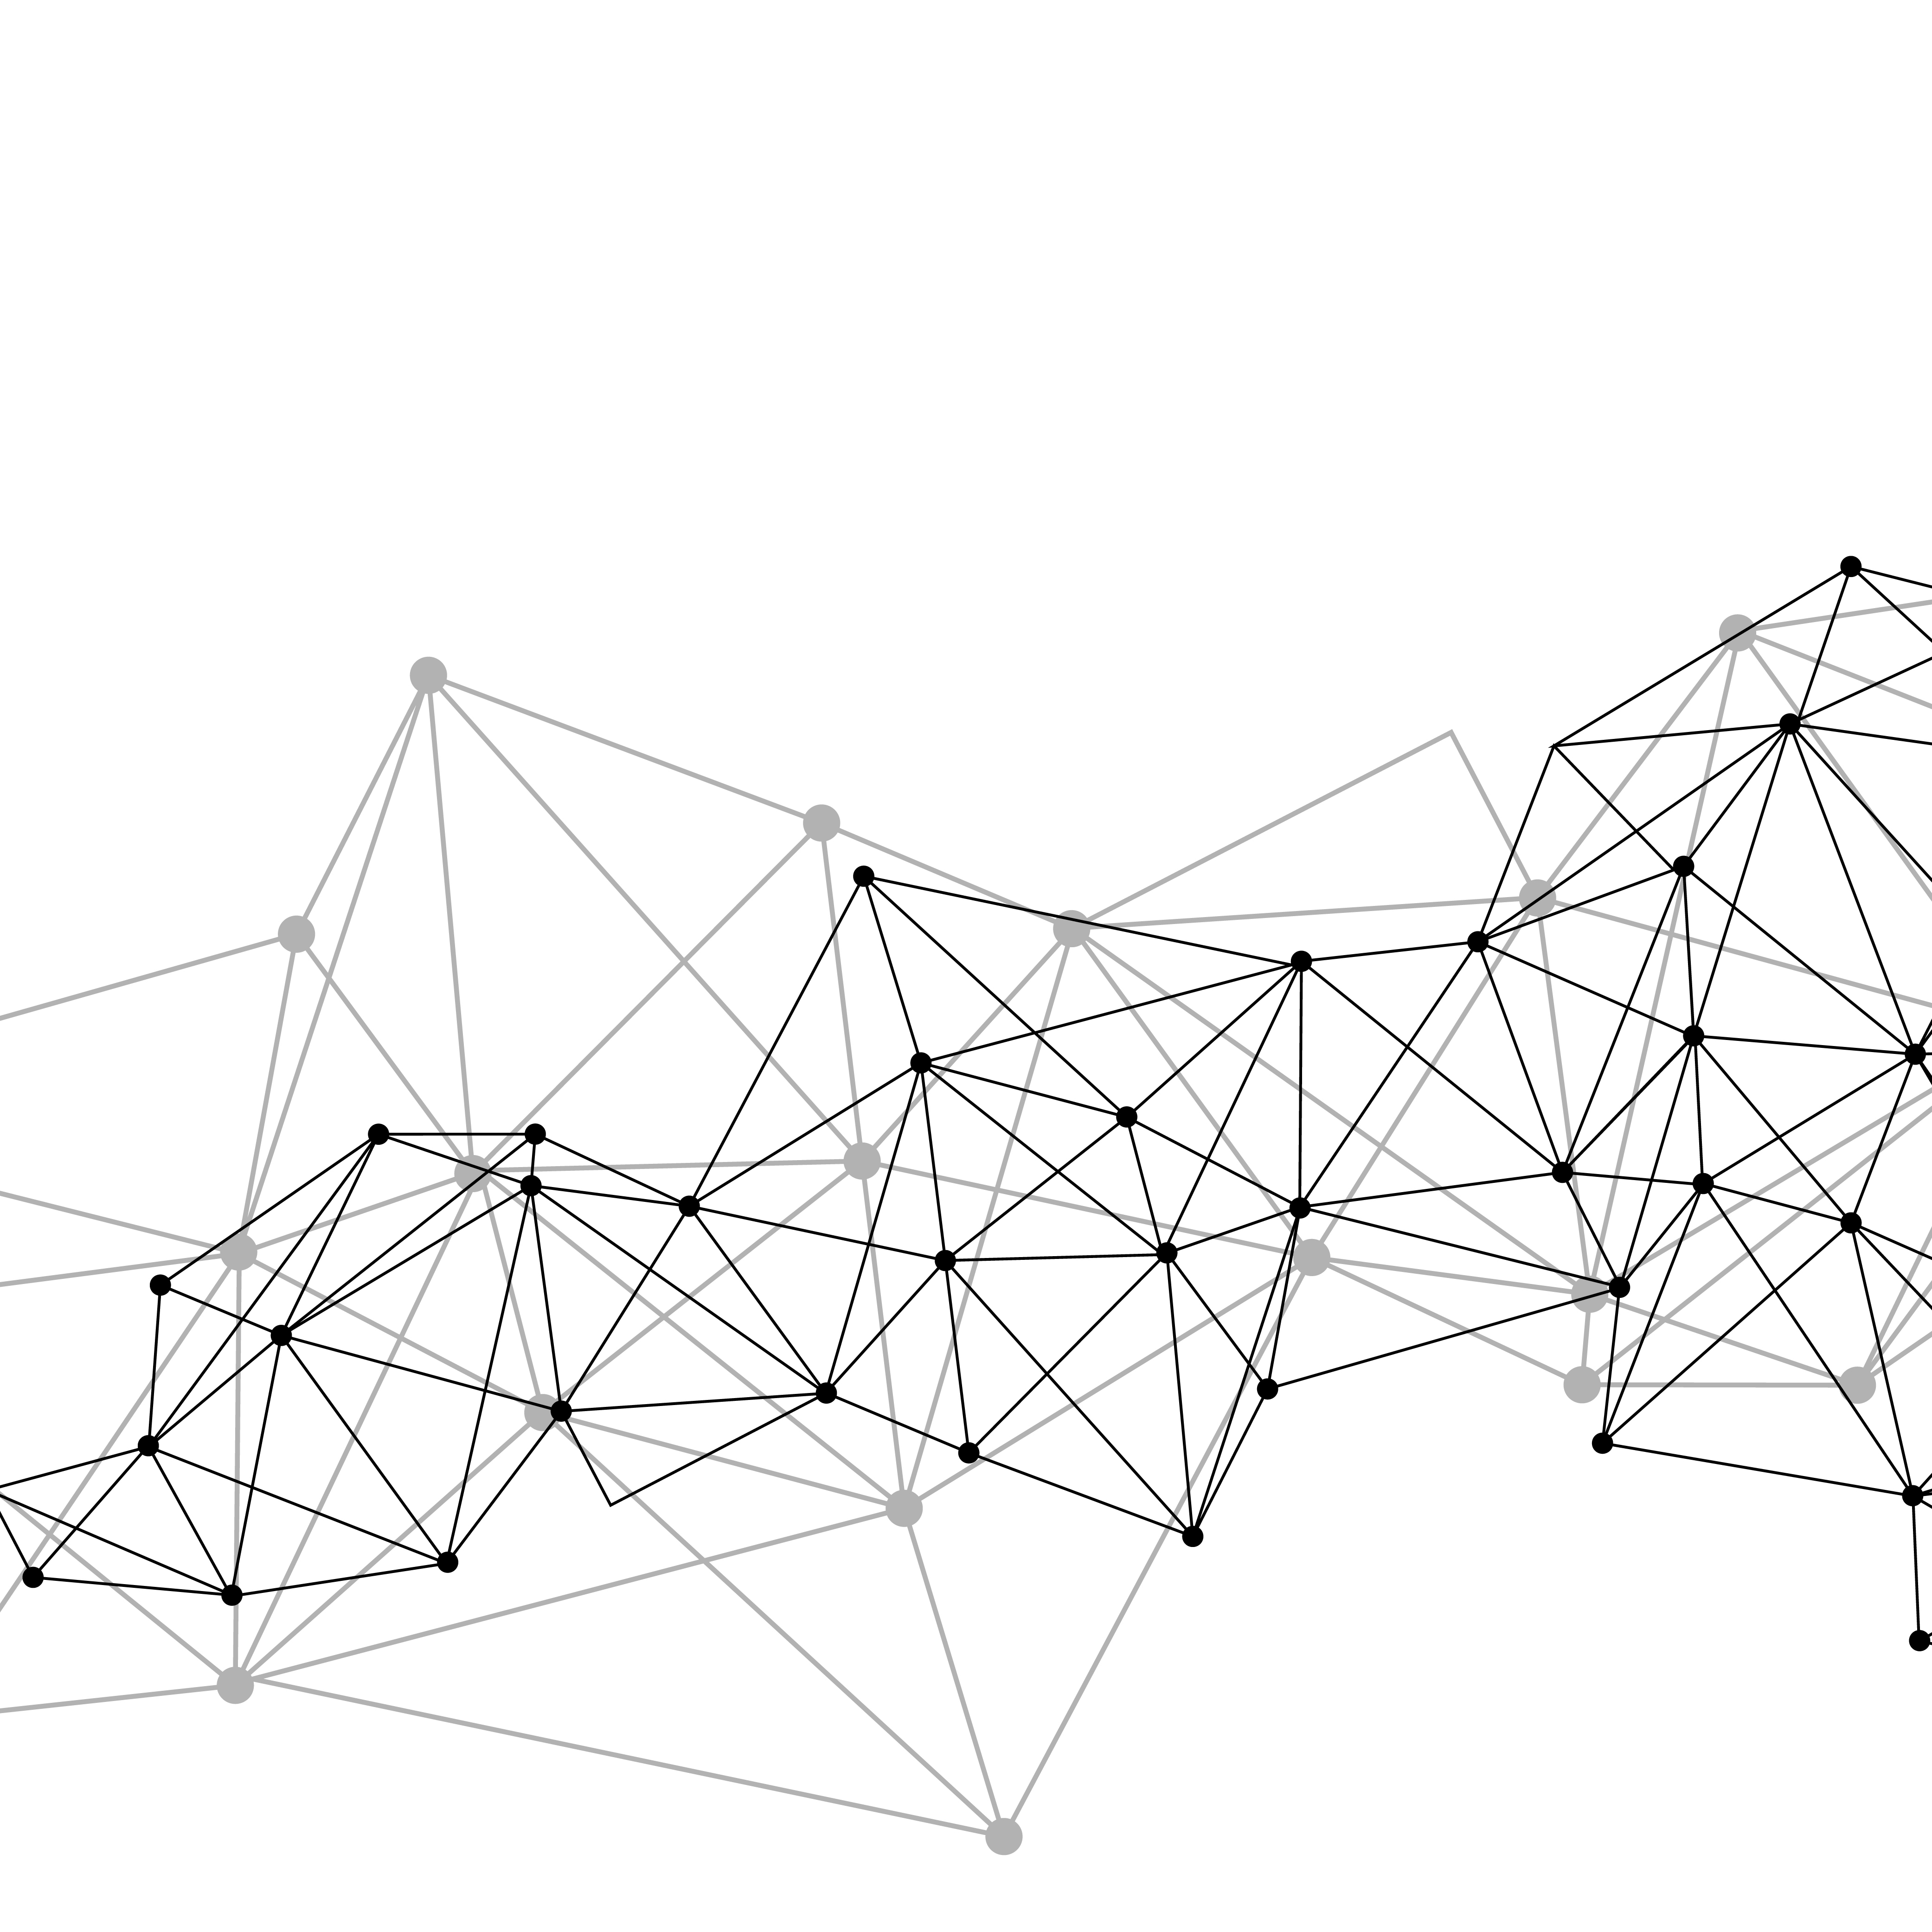
\includegraphics[width=\paperwidth]{img/main-background.jpg} 
  \end{backgroundblock} 
  \begin{card}{
    \begin{itemize}
      \item <1-> Enhance agents with \textit{some} learning capabilities 
      \item <2-> Learning improve adaptability, helping agent to act in uncertain environments
      \item <3-> Supervised Learning, Reinforcement Learning and Evolutionary Computing are typacally used in CSAS
    \end{itemize}
  }
  \end{card}
  \pause[4]
  \begin{cardRed}[\textbf{Problem} \faThumbsDown]
    \centering
    \textit{Solutions are application-specific}
  \end{cardRed}
  \pdfcomment {
    Another way of dealing with these systems is to teach them to behave properly, 
    namely by providing individual agents some learning capabilities. So, in this way, CSAS 
    can cope with challenges related to distributed sensing and decision-making and operate in uncertain environments
    Here, thanks to the new waves of interest in Machine Learning, 
    there are many insights, solutions, and ideas. 
    Reinforcement Learning, Supervised Learning, Evolutionary Computing are all tactics used in this direction. 
    Although these solutions lead to good results, they are generally very context-specific and cannot be easily applied in different situations. 
    Here we have to deal with non-stationary environments, large research space and a distributed control, which makes Machine Learning generalisation in different contexts very difficult.
  }
\end{frame}